\documentclass[../../General.tex]{subfiles}
\begin{document}


\section{Caja Negra}

Como primer paso para el modelado del diseño conceptual, es fundamental delimitar las fronteras del proyecto y comprender los elementos del sistema fotovoltaico con los que este va a interactuar. Para ello, se emplea el diagrama de Black Box, el cual permite visualizar la operación del sistema en su nivel más alto de abstracción mediante la representación de sus entradas y salidas.

En la Figura \ref{fig:caja_negra} se presenta la abstracción funcional del sistema de inspección a nivel de caja negra, la cual define las fronteras del producto y su interacción con el entorno.

\begin{figure}[H]
	\captionsetup{justification=raggedright, singlelinecheck=false, labelsep=none}
	\caption[Abstracción funcional del sistema de inspección a nivel de caja negra.]{} 
	\textit{Abstracción funcional del sistema de inspección a nivel de caja negra.} \par\medskip
	
	\makebox[\textwidth][c]{ 
		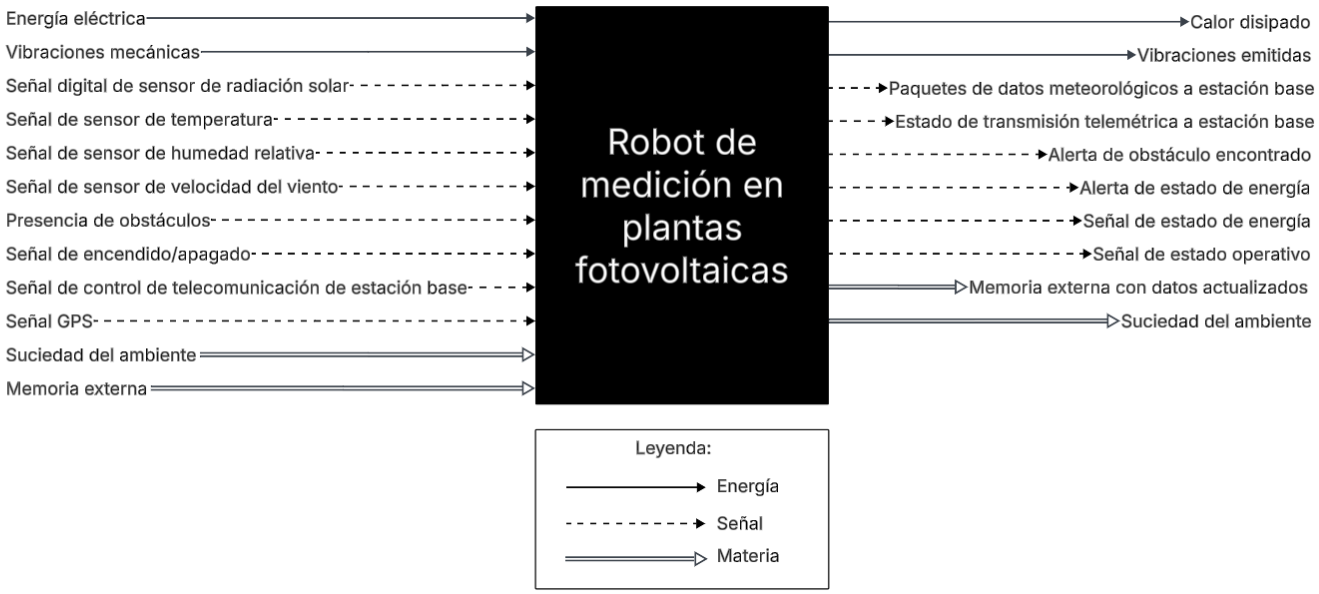
\includegraphics[width=1.2\textwidth]{Recursos/Imagenes/ImagenesDominios/A3_Blackbox_v7.png}
	} \par\medskip
	
	\raggedright
	\footnotesize \textit{Nota.} Elaboración propia.
	\label{fig:caja_negra}
\end{figure}

La función principal del sistema se define como: Transformar señales de instrumentación meteorológica externa, información espacial y comandos del usuario en paquetes de datos procesados con validez industrial y reportes de estado telemétrico.

Para cumplir con su objetivo, el sistema recibe flujos de energía de entrada compuestos por la energía eléctrica directa necesaria para su alimentación y las perturbaciones provenientes del terreno en forma de vibraciones mecánicas.

Simultáneamente, el sistema capta flujos de señales e información provenientes del entorno, las cuales incluyen la data climática (señal digital de sensor de radiación solar, señal de sensor de temperatura, señal de sensor de humedad relativa y señal de sensor de velocidad del viento), la señal GPS y la presencia de obstáculos; mientras que, desde el exterior, se introducen las instrucciones mediante la señal de encendido/apagado y la señal de control de telecomunicación de estación base.

Por otro lado, los flujos de materia que interactúan en las fronteras de entrada del sistema corresponden a la inserción física de la memoria externa y al ingreso inevitable de la suciedad del ambiente, propia de las instalaciones fotovoltaicas.

Como resultado de la transformación interna, el sistema entrega, como salidas útiles, un flujo de información compuesto por los paquetes de datos meteorológicos a estación base, el estado de transmisión telemétrica a estación base, las advertencias críticas de alerta de obstáculo encontrado y alerta de estado de energía, así como la señal de estado de energía y la señal de estado operativo requeridas para la interfaz local. Es importante destacar que estos flujos de comunicación, tanto de entrada como de salida, representan tramas de bytes estructuradas, garantizando la integridad y correcta interpretación de la telemetría.

A nivel de flujos de materia, el sistema depara la extracción de la memoria externa con datos actualizados, la cual contiene el respaldo físico de la información, y la evacuación o paso de la suciedad del ambiente.

Finalmente, como residuo del trabajo físico y computacional, el sistema libera al entorno flujos de energía en forma de calor disipado y vibraciones emitidas durante su desplazamiento continuo. Además, el sistema provee como salida un flujo de energía eléctrica para sensores meteorológicos, asegurando la alimentación y operatividad de la instrumentación externa.

\end{document}